\documentclass[12pt]{article}
\usepackage{ctex}
\usepackage[english]{babel}
\usepackage{blindtext}
\usepackage{nameref}
\usepackage{fancyhdr}
\usepackage{amsmath,amssymb,amsthm}
\usepackage{graphicx,float}
\usepackage{physics}
\usepackage{pgfplots}
\usepackage[a4paper, total={6in, 9in}]{geometry}

\graphicspath{{../picture/}}

\pagestyle{fancy}
\fancyhf{}
\fancyhf[HL]{F4 Level 5 M2 mock paper}
\fancyhf[HR]{Time limit: 1 hr 30 mins}
\fancyhf[CF]{\thepage}

\newcommand{\innerprod}[2]{\langle{#1},{#2}\rangle}
\newcommand{\id}{\mathtt{id}}

\newtheorem*{definition}{Definition}
\newtheorem*{theorem}{Theorem}
\newtheorem*{corollary}{Corollary}
\newtheorem*{lemma}{Lemma}
\newtheorem*{proposition}{Proposition}
\newtheorem*{remark}{Remark}
\newtheorem*{claim}{Claim}
\newtheorem*{example}{Example}
\newtheorem*{axiom}{Axiom}

\begin{document}
    \thispagestyle{plain}

    \centering 

    \section*{PRACTICE PAPER\\MATHEMTICS Extended Part\\Module 2 (Algebra and Calculus)\\Question-Answer Book}

    Time allowed: 1.5 hours

    Name:\hrulefill \hfill Marks:\hrulefill/100

    School:\hrulefill

    \raggedright

    \subsection*{Instructions}

    \begin{enumerate}
        \item This paper must be answered in English.
        \item Unless otherwise specified, all working must be clearly shown.
        \item Unless otherwise specified, numerical answers must be exact.
        \item This paper is for \textbf{internal use} only.
        \item All questions are collected from AL/CE/DSE past papers, reference site: https://www.dse.life/ppindex/m2/
    \end{enumerate}

    \newpage
    \begin{enumerate}
        \item (1997-CE-A MATH 2 \#07(Modified)) Let $T_n=(n^2+1)(n!)$ for any positive integer $n$. Prove, by mathematical induction, that $$\sum_{k=1}^{n}T_k=n[(n+1)!]$$for any positive integer $n$.\hfill(6 marks)
        
            \hrulefill
            
            \hrulefill
            
            \hrulefill
            
            \hrulefill
            
            \hrulefill
            
            \hrulefill
            
            \hrulefill
            
            \hrulefill
            
            \hrulefill
            
            \hrulefill
            
            \hrulefill
            
            \hrulefill
            
            \hrulefill
            
            \hrulefill
            
            \hrulefill
            
            \hrulefill
            
            \hrulefill
            
            \hrulefill
            
            \hrulefill
            
            \hrulefill
            
            \hrulefill
            
            \hrulefill
            
            \hrulefill

        \pagebreak
        \item (1988-HL-GEN MATHS \#07(Modified)) Let $$A_n=1^2-2^2+3^2-4^2+\dots+(-1)^{n-1}n^2$$ and $$B_n=1+2+3+\dots+n=\frac{n(n+1)}{2}$$ where $n$ is a positive integer.\begin{enumerate}
            \item Show, by mathematical induction, that $A_n=(-1)^{n-1}B_n$ for all positive integer $n$.
            \item Hence, or otherwise, find $\displaystyle\sum_{n=1}^{2m}A_n$ and $\displaystyle\sum_{n=1}^{2m+1}A_n$.
        \end{enumerate}\hfill(8 marks)
        
            \hrulefill
            
            \hrulefill
            
            \hrulefill
            
            \hrulefill
            
            \hrulefill
            
            \hrulefill
            
            \hrulefill
            
            \hrulefill
            
            \hrulefill
            
            \hrulefill
            
            \hrulefill
            
            \hrulefill
            
            \hrulefill
            
            \hrulefill
            
            \hrulefill
            
            \hrulefill
            
            \hrulefill
            
            \hrulefill
            
            \hrulefill
            
            \hrulefill
            
            \hrulefill
            
            \hrulefill
            
            \hrulefill
            
            \hrulefill
            
            \hrulefill
            
            \hrulefill
            
            \hrulefill
            
            \hrulefill
            
            \hrulefill
            
            \hrulefill
            
            \hrulefill
            
            \hrulefill
            
            \hrulefill
            
            \hrulefill
            
            \hrulefill
            
            \hrulefill
            
            \hrulefill
            
            \hrulefill
            
            \hrulefill
            
            \hrulefill
            
            \hrulefill
            
            \hrulefill
            
            \hrulefill
            
            \hrulefill
            
            \hrulefill
            
            \hrulefill

        \pagebreak
        \item (2017-DSE-MATH-EP(M2) \#02) Let $\displaystyle (1+ax)^8=\sum_{k=0}^8 \lambda_k x^k$ and $\displaystyle(b+x)^9=\sum_{k=0}^9 \mu_k x^k$, where $a$ and $b$ are constants. It is given that $\lambda_2:\mu_7=7:4$ and $\lambda_1+\mu_8+6=0$. Find $a$.\hfill(6 marks)
        
        \hrulefill
            
        \hrulefill
        
        \hrulefill
        
        \hrulefill
        
        \hrulefill
        
        \hrulefill
        
        \hrulefill
        
        \hrulefill
        
        \hrulefill
        
        \hrulefill
        
        \hrulefill
        
        \hrulefill
        
        \hrulefill
        
        \hrulefill
        
        \hrulefill
        
        \hrulefill
        
        \hrulefill
        
        \hrulefill
        
        \hrulefill
        
        \hrulefill
        
        \hrulefill
        
        \hrulefill
        
        \hrulefill
        
        \hrulefill

    \pagebreak
        \item (1989-HL-GEN MATHS \#05(Modified))  \begin{enumerate}
            \item Find the solution of $\sin{x}-\sin{2x}+\sin{3x}=0$ for $0<x<2\pi$.
            \item Let $f(\theta)=\sin{2\theta}+\sin{\theta}+\cos{\theta}$.\begin{enumerate}
                \item Express $f(\theta)$ in terms of $p$, where $p=\sin{\theta}+\cos{\theta}$.
                \item Using (i) and the method of completing the square, find the smallest value of $f(\theta)$. For $0<\theta<\pi$, find also the value of $\theta$ such that $f(\theta)$ attains its smallest value.
            \end{enumerate}
        \end{enumerate}\hfill(18 marks)

        \hrulefill
            
            \hrulefill
            
            \hrulefill
            
            \hrulefill
            
            \hrulefill
            
            \hrulefill
            
            \hrulefill
            
            \hrulefill
            
            \hrulefill
            
            \hrulefill
            
            \hrulefill
            
            \hrulefill
            
            \hrulefill
            
            \hrulefill
            
            \hrulefill
            
            \hrulefill
            
            \hrulefill
            
            \hrulefill
            
            \hrulefill
            
            \hrulefill
            
            \hrulefill
            
            \hrulefill
            
            \hrulefill
            
            \hrulefill
            
            \hrulefill

            \hrulefill
            
            \hrulefill
            
            \hrulefill
            
            \hrulefill
            
            \hrulefill
            
            \hrulefill
            
            \hrulefill
            
            \hrulefill
            
            \hrulefill
            
            \hrulefill
            
            \hrulefill
            
            \hrulefill
            
            \hrulefill
            
            \hrulefill
            
            \hrulefill
            
            \hrulefill
            
            \hrulefill
            
            \hrulefill
            
            \hrulefill
            
            \hrulefill
            
            \hrulefill
            
            \hrulefill
            
            \hrulefill
            
        \pagebreak
        \item (1984-HL GEN MATHS \#05(Modified)) \begin{enumerate}
            \item Express $\cot{4\theta}$ in terms of $\cot{\theta}$. Hence solve the equation $x^4-4x^3-6x^2+4x+1=0$. (Give your answers in terms of $\pi$.)
            \item \begin{enumerate}
                \item If $\cos{\theta}-\cos{\phi}=a$ and $\sin{\theta}-\sin{\phi}=b$ $(b\neq 0)$, show that $$\frac{1}{2}(2-a^2-b^2)=\cos{\theta-\phi}\textrm{ and }\frac{-a}{b}=\tan{\frac{\theta+\phi}{2}}.$$
                \item Solve the system of equations $$\begin{cases}
                    \cos{\theta}-\cos{\phi}=1\\
                    \sin{\theta}-\sin{\phi}=\sqrt{3}
                \end{cases}$$
                where $0\leq \theta \leq 2\pi$ and $0\leq \phi \leq 2\pi$.
            \end{enumerate}
        \end{enumerate}\hfill(18 marks)

        \hrulefill
            
            \hrulefill
            
            \hrulefill
            
            \hrulefill
            
            \hrulefill
            
            \hrulefill
            
            \hrulefill
            
            \hrulefill
            
            \hrulefill
            
            \hrulefill
            
            \hrulefill
            
            \hrulefill
            
            \hrulefill
            
            \hrulefill
            
            \hrulefill
            
            \hrulefill
            
            \hrulefill
            
            \hrulefill
            
            \hrulefill
            
            \hrulefill
            
            \hrulefill
            
            \hrulefill

            \hrulefill
            
            \hrulefill
            
            \hrulefill
            
            \hrulefill
            
            \hrulefill
            
            \hrulefill
            
            \hrulefill
            
            \hrulefill
            
            \hrulefill
            
            \hrulefill
            
            \hrulefill
            
            \hrulefill
            
            \hrulefill
            
            \hrulefill
            
            \hrulefill
            
            \hrulefill
            
            \hrulefill
            
            \hrulefill
            
            \hrulefill
            
            \hrulefill
            
            \hrulefill
            
            \hrulefill
            
            \hrulefill
            
        \pagebreak
        \item (2018-DSE-MATH-EP(M2) \#01) Let $f(x)=(x^2-1)e^x$. Express $f(1+h)$ in terms of $h$. Hence, find $f'(1)$ from first principles.\hfill(6 marks)
        
        \hrulefill
            
            \hrulefill
            
            \hrulefill
            
            \hrulefill
            
            \hrulefill
            
            \hrulefill
            
            \hrulefill
            
            \hrulefill
            
            \hrulefill
            
            \hrulefill
            
            \hrulefill
            
            \hrulefill
            
            \hrulefill
            
            \hrulefill
            
            \hrulefill
            
            \hrulefill
            
            \hrulefill
            
            \hrulefill
            
            \hrulefill
            
            \hrulefill
            
            \hrulefill
            
            \hrulefill
            
            \hrulefill

        \pagebreak
        \item (PP-DSE-MATH-EP(M2) \#07) Let $f(x)=e^x(\sin{x}+\cos{x})$.\begin{enumerate}
            \item Find $f'(x)$ and $f''(x)$.
            \item Solve for $x$ when $f''(x)-f'(x)+f(x)=0$, where $x$ is real number.
        \end{enumerate}\hfill(8 marks)
        
        \hrulefill
            
            \hrulefill
            
            \hrulefill
            
            \hrulefill
            
            \hrulefill
            
            \hrulefill
            
            \hrulefill
            
            \hrulefill
            
            \hrulefill
            
            \hrulefill
            
            \hrulefill
            
            \hrulefill
            
            \hrulefill
            
            \hrulefill
            
            \hrulefill
            
            \hrulefill
            
            \hrulefill
            
            \hrulefill
            
            \hrulefill
            
            \hrulefill
            
            \hrulefill
            
            \hrulefill

        \pagebreak
        \item (1996-CE-A MATH 1 \#06) Find the equations of the two tangents to the curve $C:y=\dfrac{6}{x+1}$ which are parallel to the line $x+6y+10=0$.\hfill(7 marks)
        
        \hrulefill
            
            \hrulefill
            
            \hrulefill
            
            \hrulefill
            
            \hrulefill
            
            \hrulefill
            
            \hrulefill
            
            \hrulefill
            
            \hrulefill
            
            \hrulefill
            
            \hrulefill
            
            \hrulefill
            
            \hrulefill
            
            \hrulefill

            \hrulefill
            
            \hrulefill
            
            \hrulefill
            
            \hrulefill
            
            \hrulefill
            
            \hrulefill
            
            \hrulefill
            
            \hrulefill
            
            \hrulefill
            
            \hrulefill

        \pagebreak
        \item (1994-CE-A MATH 1 \#12) 
        \begin{figure}[H]
            \centering
            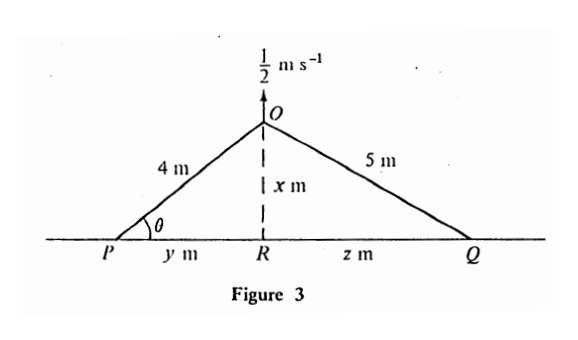
\includegraphics[scale=1.4]{1994CE_A_MATH_1_12.png}
        \end{figure}
        In figure 3, two rods $OP$ and $OQ$ are hinged at $O$. The lengths of $OP$ and $OQ$ are 4 m and 5 m respectively. The end $O$ is pushed upwards at a constant rate of $\dfrac{1}{2}$ ms$^{-1}$ along a fixed vertical axis, and the ends $P$ and $Q$ move along a horizontal rail. $R$ is the projection of $O$ on the rail. At time $t$ seconds, $OR = x$ m and $\angle OPQ=\theta$ where $0<\theta<\dfrac{\pi}{2}$.\begin{enumerate}
            \item \begin{enumerate}
                \item Express $x$ in terms of $\theta$. 
                \item Hence find the rate of change of $\theta$ with respect to $t$ in terms of $\theta$.
            \end{enumerate}
            \item Let $PR=y$ m,$RQ=z$ m.\begin{enumerate}
                \item Express $\dfrac{dy}{dt}$ and $\dfrac{dz}{dt}$ in terms of $\theta$.
                \item Hence find the rate of change of $PQ$ with respect to $t$ when $\theta=\dfrac{\pi}{6}$, giving your answer correct to 3 significant figures.
            \end{enumerate}
            \item \begin{enumerate}
                \item Find the value of $\theta$ such that the area of $\triangle OPR$ is a maximum.
                \item By considering the value of $\angle OQR$, find the value of $\theta$ such that the area of $\triangle ORQ$ is a maximum, giving your answer correct to 3 significant figures. 
            \end{enumerate} 
        \end{enumerate}\hfill(23 marks)

        \hrulefill
            
            \hrulefill
            
            \hrulefill
            
            \hrulefill
            
            \hrulefill
            
            \hrulefill
            
            \hrulefill
            
            \hrulefill
            
            \hrulefill
            
            \hrulefill
            
            \hrulefill
            
            \hrulefill
            
            \hrulefill

            \hrulefill
            
            \hrulefill
            
            \hrulefill
            
            \hrulefill
            
            \hrulefill
            
            \hrulefill
            
            \hrulefill
            
            \hrulefill
            
            \hrulefill
            
            \hrulefill

            \hrulefill
            
            \hrulefill
            
            \hrulefill
            
            \hrulefill
            
            \hrulefill
            
            \hrulefill
            
            \hrulefill
            
            \hrulefill
            
            \hrulefill
            
            \hrulefill
            
            \hrulefill
            
            \hrulefill
            
            \hrulefill

            \hrulefill
            
            \hrulefill
            
            \hrulefill
            
            \hrulefill
            
            \hrulefill
            
            \hrulefill
            
            \hrulefill
            
            \hrulefill
            
            \hrulefill
            
            \hrulefill

            \hrulefill
            
            \hrulefill
            
            \hrulefill
            
            \hrulefill
            
            \hrulefill
            
            \hrulefill
            
            \hrulefill
            
            \hrulefill
            
            \hrulefill
            
            \hrulefill
            
            \hrulefill
            
            \hrulefill
            
            \hrulefill

            \hrulefill
            
            \hrulefill
            
            \hrulefill
            
            \hrulefill
            
            \hrulefill
            
            \hrulefill
            
            \hrulefill
            
            \hrulefill
            
            \hrulefill
            
            \hrulefill

            \hrulefill
            
            \hrulefill
            
            \hrulefill
            
            \hrulefill
            
            \hrulefill
            
            \hrulefill
            
            \hrulefill
            
            \hrulefill
            
            \hrulefill
            
            \hrulefill
            
            \hrulefill
            
            \hrulefill
            
            \hrulefill
            
            \hrulefill
            
            \hrulefill

        \pagebreak
    \end{enumerate}
\end{document}